%%%%%%%%% JPS abstract %%%%%%%%%%%%%%%%%%%%%%%%%%%%%%%%%%%%%%%%%%
\documentclass[12pt,a4paper,upLaTeX]{jsarticle}

%%%%%%%%% packages %%%%%%%%%%%%%%%%%%%%%%%%%%%%%%%%%%%%%%%%%%%%%%
\usepackage[dvipdfmx]{graphicx} % Include figure files
\usepackage[%                           % 余白の設定
%mag=1400,%                              jarticle の場合（14ptに）
dvipdfm,truedimen,%
top=30truemm,bottom=50truemm,%
left=20truemm,right=20truemm]{geometry}
\usepackage{fancyhdr}
\usepackage{amsmath,amssymb}
\usepackage{bm}
\pagestyle{fancy}

%%%%%%%%% header %%%%%%%%%%%%%%%%%%%%%%%%%%%%%%%%%%%%%%%%%%%%%%%%
\begin{document}

\fancyhf{}
\setlength{\headheight}{60pt}   % ある程度大きめに
\fancyhead[R]{大阪大学大学院 理学研究科 物理学専攻 博士前期課程2年\\
学籍番号 24B25011\\
加島 駿一\\}

\setlength{\footskip}{20pt}
% \fancyhf{}
\fancyfoot[C]{CUDA programming get started memo}

\fancyfoot[R]{\thepage}

\vspace{50pt}
\begin{center}
{\gt \Large MEMO: Nvidia CUDA programming get started }\\[14pt]

\end{center}

\vspace{10pt}
%%%%%%%%%%%%%%%%%%%%%%%%%%%%%%%%%%%%%%%%%%%%%%%%%%

\subsubsection*{CUDA Programming Guide}
\begin{itemize}
  \item CPU/GPUをホスト/デバイスと呼び分けている
  \item CUDA APIを通してホストメモリからデバイスメモリにデータをコピーすることができる
  \item Graphics Processing Clusters(GPCs)はStreaming Multiprocessors(SMs)の集まり
  \item SMはa local register fileとa unified data cacheと計算を行なう多数の機能ユニットを持つ
  \item 統合データキャッシュは共有メモリとL1キャッシュの実体である
  \begin{itemize}
    \item 統合データキャッシュ -> (共有メモリ, L1キャッシュ)への割り当ては実行時に設定できる
  \end{itemize}
\end{itemize}


\begin{figure}[tbhp]
  \centering
  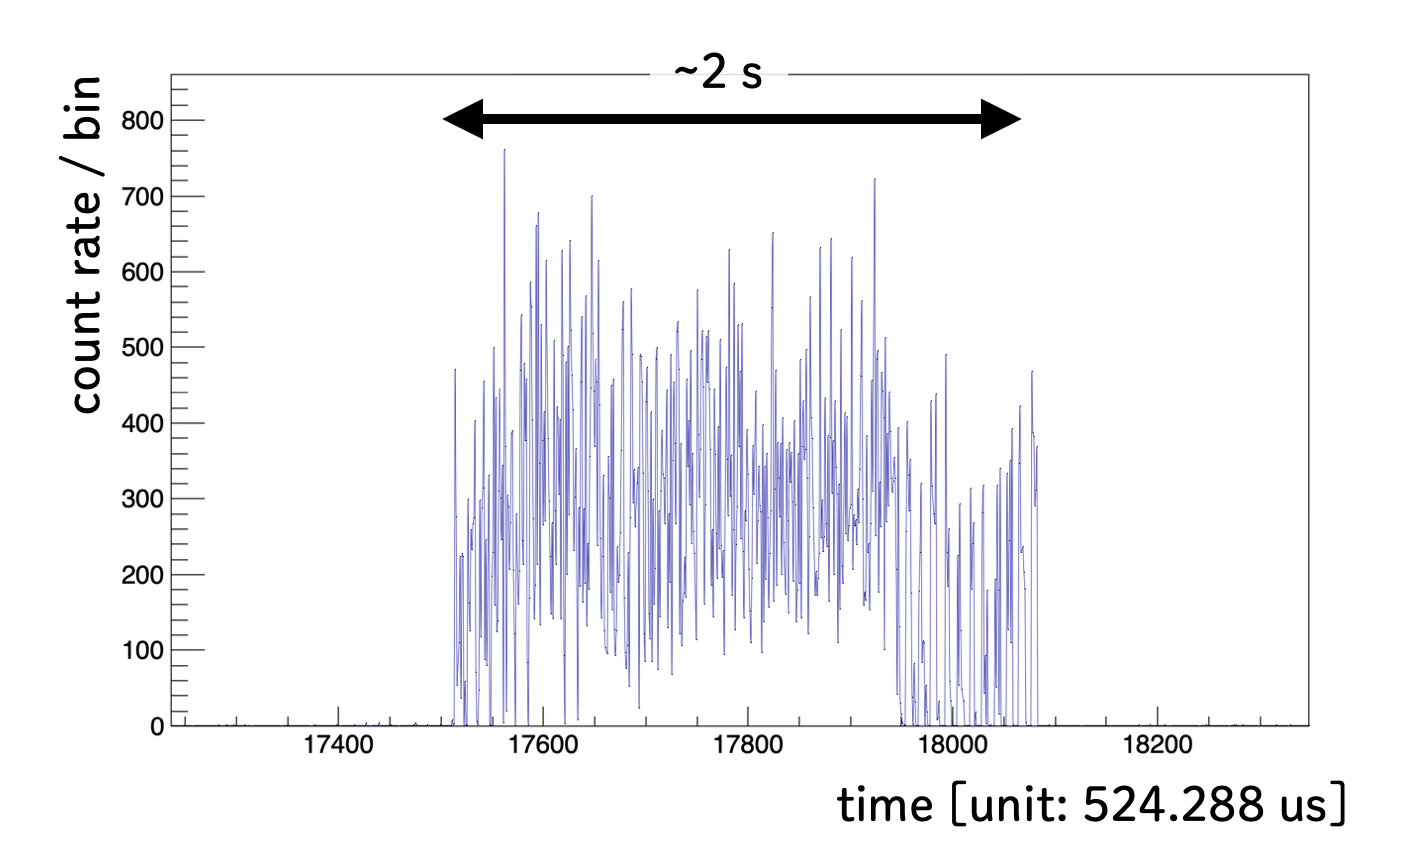
\includegraphics[width=0.8\textwidth]{./PICTURE/beam_structure.png}
  \caption{J-PARC ハドロン実験施設に供給されるビームの時間的な構造の例。約2秒の間、加速器施設のメインリングから徐々にビームを取り出すSlow extractionと呼ばれる方式でビームを検出器に照射している。横軸は時間で、縦軸は検出器のカウントレートである。}
  \label{fig:beam_structure}
\end{figure}

% J-PARCにあるハドロン実験施設に供給されるSlow extractionビームを用いる


\end{document}